\subsection{Lab23: BER}

%*********************
\begin{frame}{}

\pgfdeclareimage[width=\paperwidth,height=\paperheight]{bg}{imagenes/fondo_lab}
\setbeamertemplate{background}{\pgfuseimage{bg}}

\bfseries{\textrm{\LARGE Lab23\\ \Large BER}}
\raggedright
\end{frame}
%*************
%----------------------------------------

%_---------------------
%_---------------------
\begin{frame}
\pgfdeclareimage[width=\paperwidth,height=\paperheight]{bg}{imagenes/fondo3}
\setbeamertemplate{background}{\pgfuseimage{bg}}

\frametitle{\underline{\textbf{BER}}}

  \begin{center}
  \textbf{BER}
  \end{center}
  
  \begin{flushleft}
  La tasa de error de bit (BER) es el número de errores de bit por unidad de tiempo. La relación de error de bit (también BER) es el número de errores de bit dividido por el número total de bits transferidos durante un intervalo de tiempo. La relación de error de bit es una medida de rendimiento sin unidades.
  \end{flushleft}
  
\end{frame} 
%_---------------------
%_--------------------- 
 
\begin{frame} 
\pgfdeclareimage[width=\paperwidth,height=\paperheight]{bg}{imagenes/fondo3}
\setbeamertemplate{background}{\pgfuseimage{bg}}

\frametitle{\underline{\textbf{BER}}}
  \begin{flushleft}
  {En GNU Radio para calcular la tasa de error en un modulación utilizamos el siguiente diagrama}
  \end{flushleft}
  \begin{figure}[H]
  \vspace{-3mm}
  \centering
  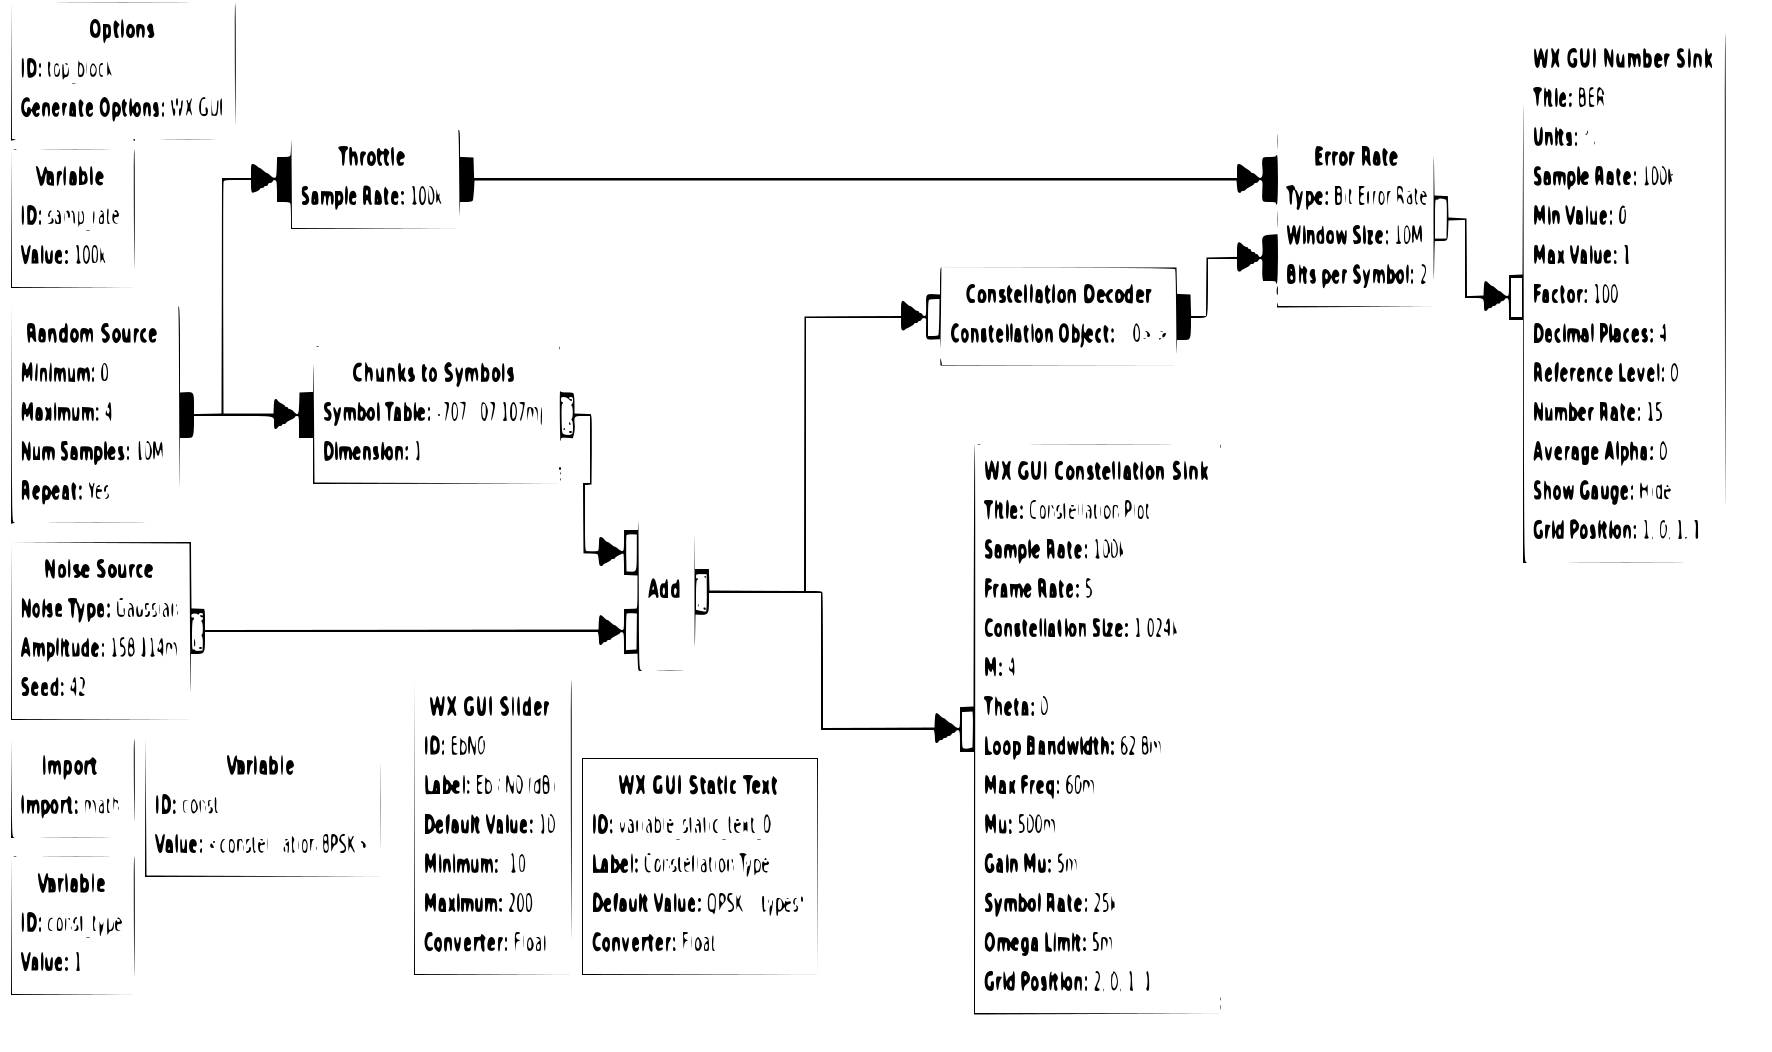
\includegraphics[width=0.8\textwidth]{Modulaciones_digitales/lab23/pdf/BER_1.pdf}
  \end{figure}
\end{frame}  

%_---------------------
%_---------------------

\begin{frame}
\begin{figure}[H]
\vspace{-3mm}
\centering
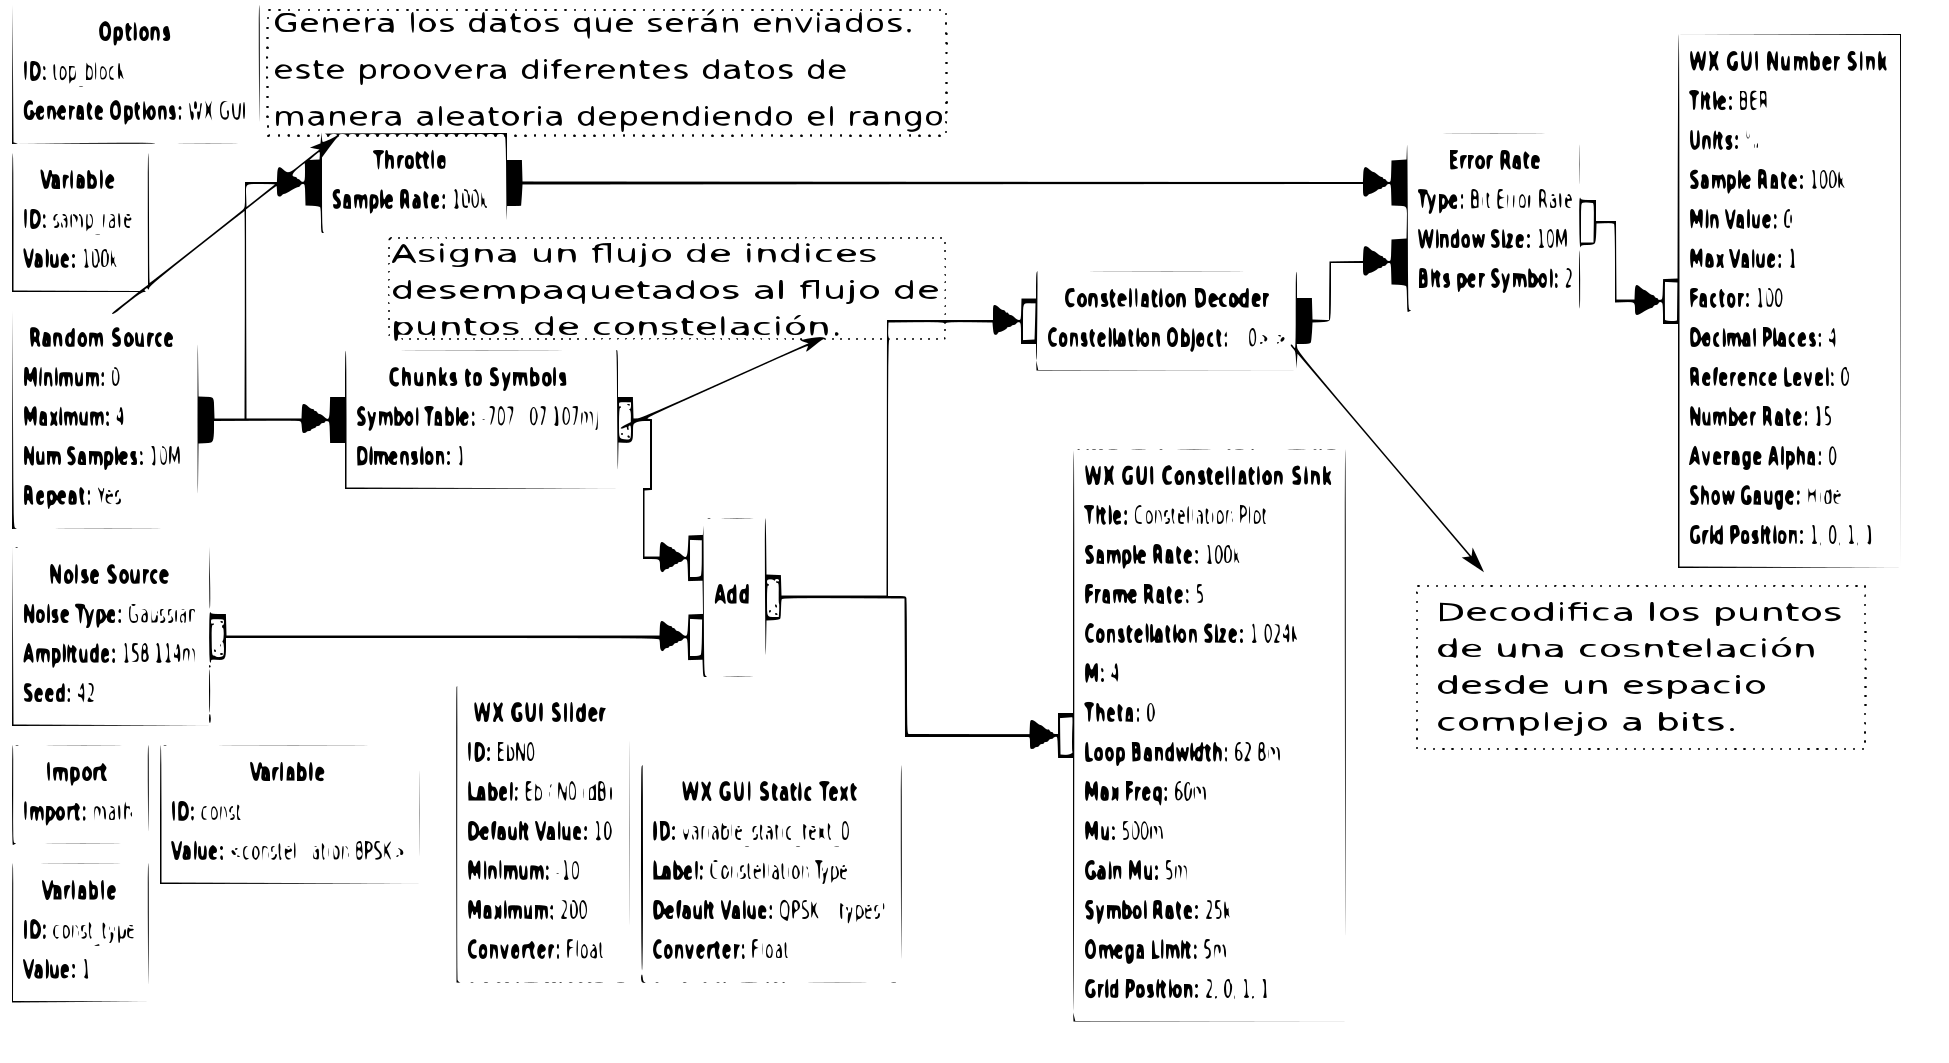
\includegraphics[width=1\textwidth]{Modulaciones_digitales/lab23/pdf/BER_2.pdf}
\end{figure}
\end{frame}

%_---------------------
%_---------------------

\begin{frame}
\begin{figure}[H]
\vspace{-3mm}
\centering
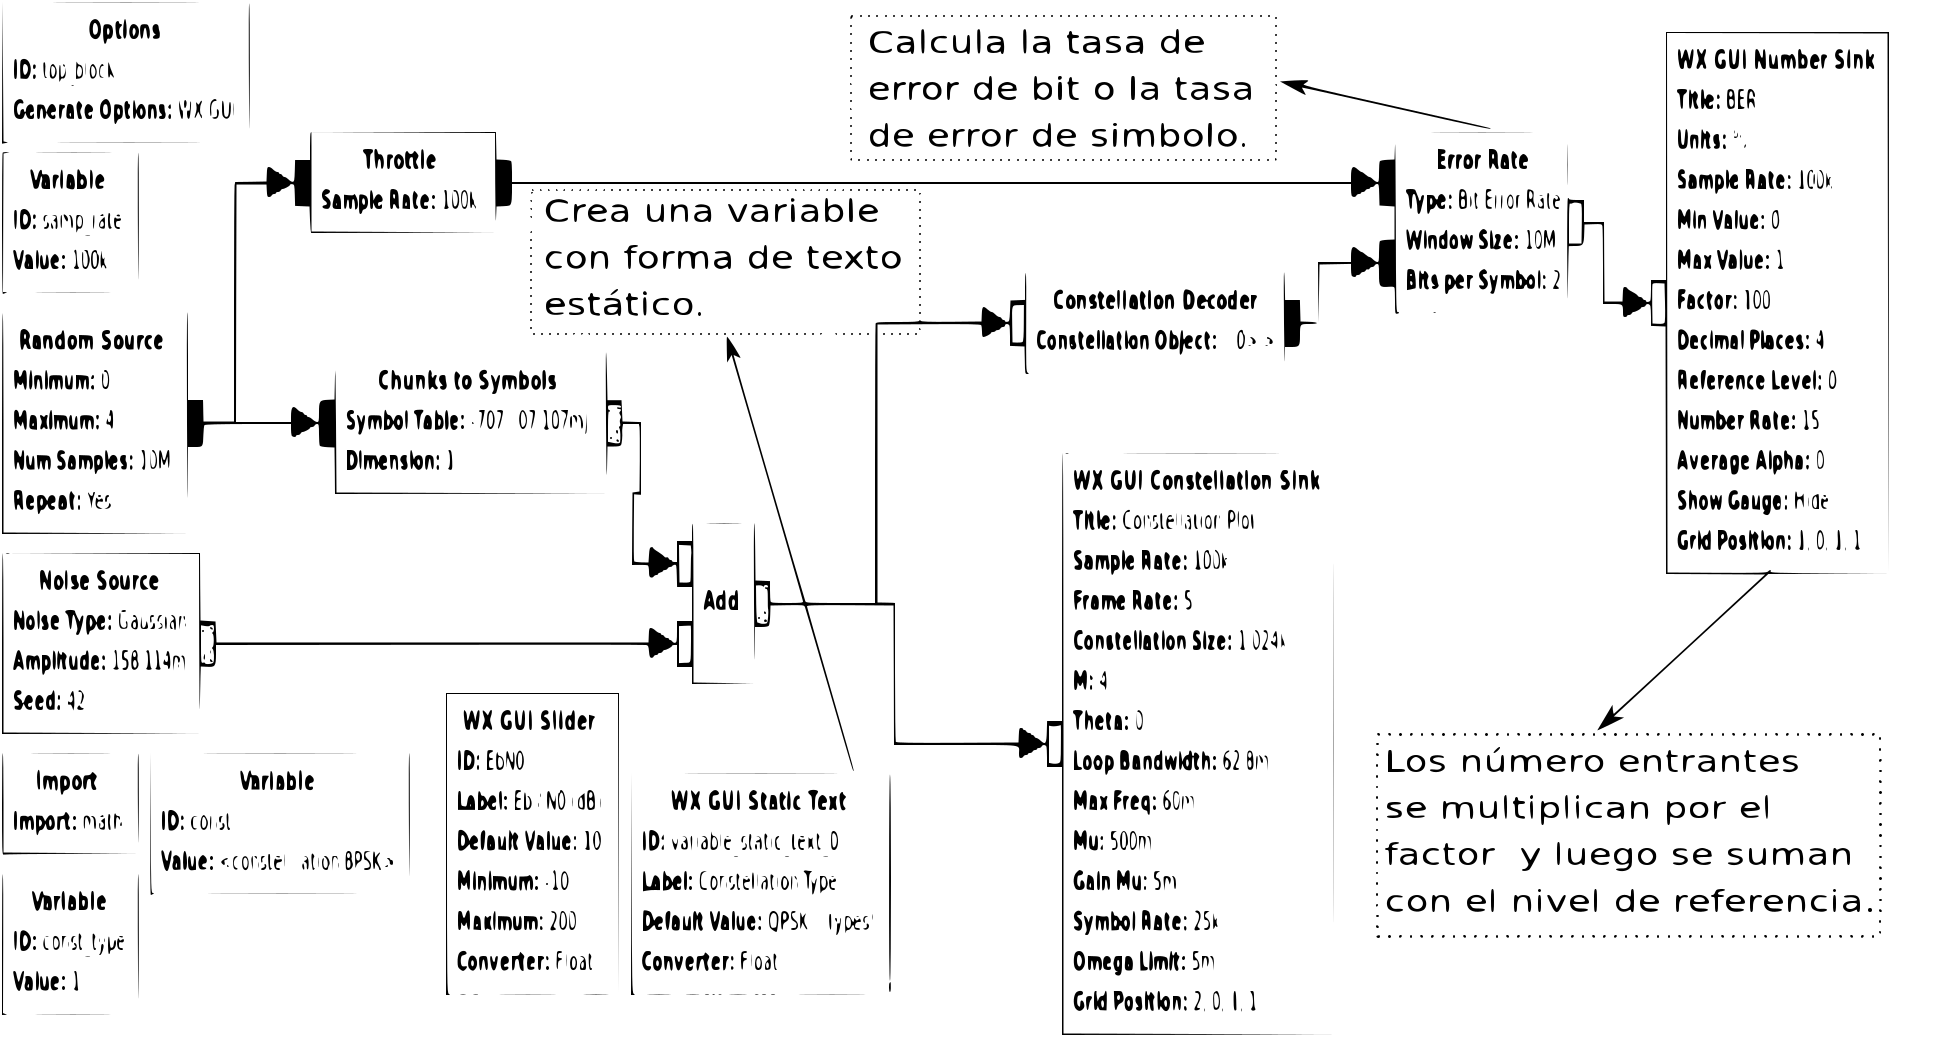
\includegraphics[width=1\textwidth]{Modulaciones_digitales/lab23/pdf/BER_3.pdf}
\end{figure}
\end{frame}

%_---------------------
%_---------------------

\begin{frame}
\pgfdeclareimage[width=\paperwidth,height=\paperheight]{bg}{imagenes/fondo3}
\setbeamertemplate{background}{\pgfuseimage{bg}}

\frametitle{\underline{\textbf{BER}}}
\begin{itemize}
    \item {Agregue una variable "consttype" y establezca su valor en: 1}
    \item {Agregue una nueva variable "const", y establezca su valor en:(digital.constellationbpsk (),digital.constellationqpsk (),digital.constellation8psk ()) }
    \item {En el lado derecho, busque "Random Source" en la categoría "Sources". Haga doble clic en el bloque "Fuente aleatoria" y cambie el tipo de salida a "Byte", el máximo a. Constelación es el nombre del objeto de constelación GnuRadio y número de muestras a 10M (intente usar int (10e6) en lugar de 1000000) .}
\end{itemize}
\end{frame}

%_---------------------
%_---------------------

\begin{frame}
\begin{figure}[H]
\vspace{-3mm}
\centering
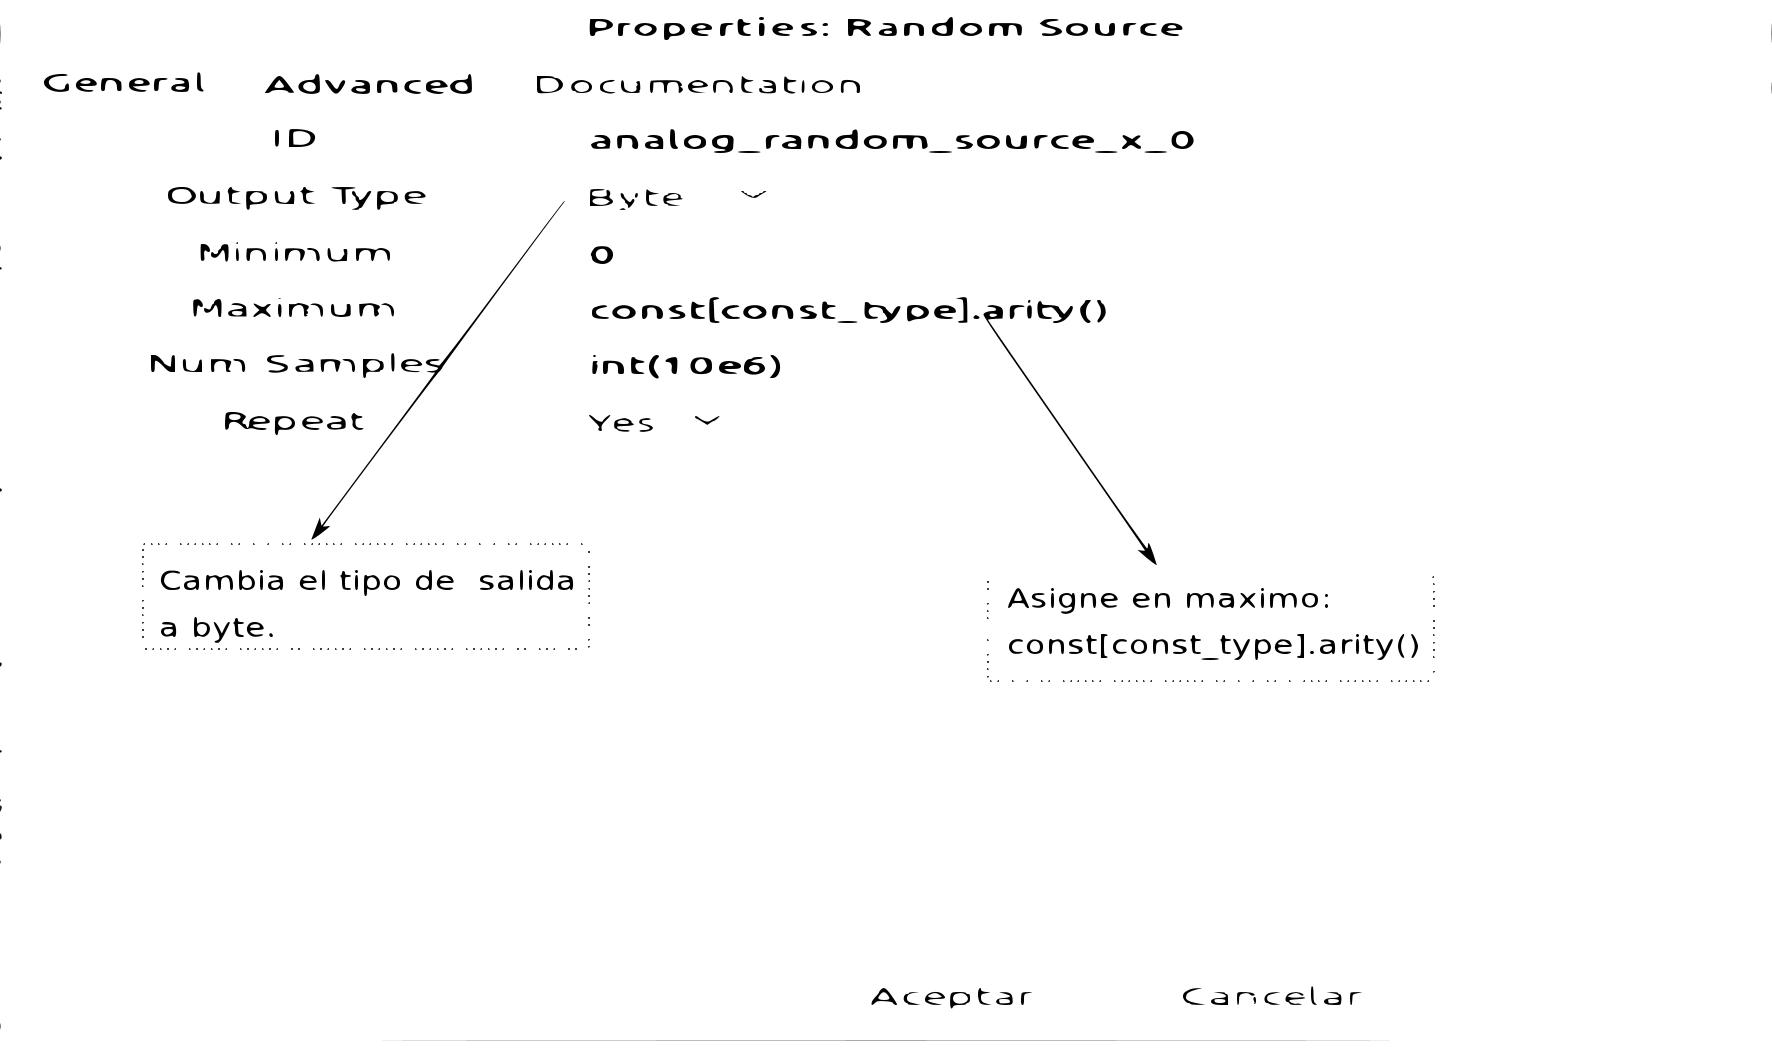
\includegraphics[width=0.9\textwidth]{Modulaciones_digitales/lab23/pdf/randomber.pdf}
\end{figure}
\end{frame}

%_---------------------
%_---------------------

\begin{frame}
\pgfdeclareimage[width=\paperwidth,height=\paperheight]{bg}{imagenes/fondo3}
\setbeamertemplate{background}{\pgfuseimage{bg}}

\frametitle{\underline{\textbf{BER}}}
    \begin{itemize}
        \item{Agrege un "WX Static Text"}
    \end{itemize}
\begin{figure}[H]
\vspace{-3mm}
\centering
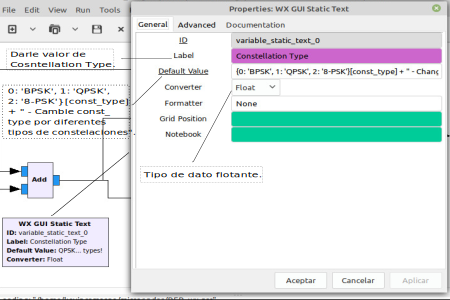
\includegraphics[width=1\textwidth]{Modulaciones_digitales/lab23/pdf/statictex.pdf}
\end{figure}
\end{frame}

%_---------------------
%_---------------------

\begin{frame}
\pgfdeclareimage[width=\paperwidth,height=\paperheight]{bg}{imagenes/fondo3}
\setbeamertemplate{background}{\pgfuseimage{bg}}

\frametitle{\underline{\textbf{BER}}}
\begin{itemize}
    \item {Agregue WX GUI Slider, valores mínimos establecidos en -100, valor máximo establecido en 100, valores predeterminados establecidos en 10. Nombre "EbN0"
este control deslizante como "EbN0" (ID de objeto).}
\item{Importar una biblioteca "math" (componente "Import", valor: "import math")}
\item{Agregue "Noise source" de la categoría "Sources" y cambie la amplitud como
1.0 / math.sqrt (2.0 * const [consttype] .bitspersymbol () * 10 ** (EbN0 / 10)).}
   \item{Agregue "Chunks to symbols" de la categoría "Misc Conversion" y cambie el tipo de entrada a "Byte", tabla de símbolos para "const [consttype] .points ()", la dimensión a 1.}
\end{itemize}
\end{frame}

%_---------------------
%_---------------------

\begin{frame}
\begin{figure}[H]
\vspace{-3mm}
\centering
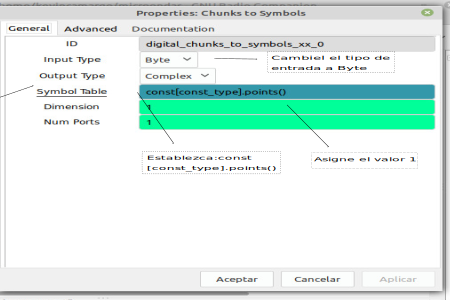
\includegraphics[width=1\textwidth]{Modulaciones_digitales/lab23/pdf/Chuckto.pdf}
\end{figure}
\end{frame}

%_---------------------
%_---------------------

\begin{frame}
\begin{itemize}
    \item {Agregue “Add” de la categoría “Operadores” y haga conexiones entre “Chunks to Symbols" y " Noise Source ".}
    \item{Agregue "WX Constellation Sink" de la categoría " y realice conexiones entre este componente y el componente "Add".}
    \item{Agregue "Constellation Decoder" Establezca en Constellation Object: const [tipoconst] .base (). 
    Conecte a su entrada el componente "Add" }
\end{itemize}
\end{frame}

%_---------------------
%_---------------------

\begin{frame}
\begin{figure}[H]
\vspace{-3mm}
\centering
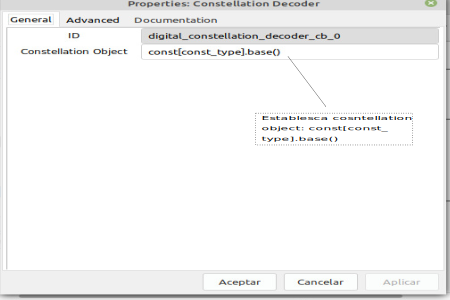
\includegraphics[width=1\textwidth]{Modulaciones_digitales/lab23/pdf/Decoder.pdf}
\end{figure}
\end{frame}

%_---------------------
%_---------------------

\begin{frame}
\begin{itemize}
\item{Agregue "Error Rate"  y cambie el tamaño de la ventana a 10M (int (1e7)), el Bits per símbol a "const[consttype].bitspersymbol ())".}
\end{itemize}
\begin{figure}[H]
\vspace{-3mm}
\centering
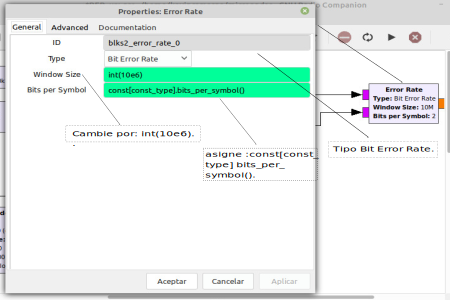
\includegraphics[width=1\textwidth]{Modulaciones_digitales/lab23/pdf/errorrate.pdf}
\end{figure}
\end{frame}

%_---------------------
%_---------------------

\begin{frame}
    \begin{itemize}
        \item {Agregue "WX Number Sink". Establezca la entrada en flotante, min a 0 y max a 1.}
\end{itemize}
\begin{figure}[H]
\vspace{-3mm}
\centering
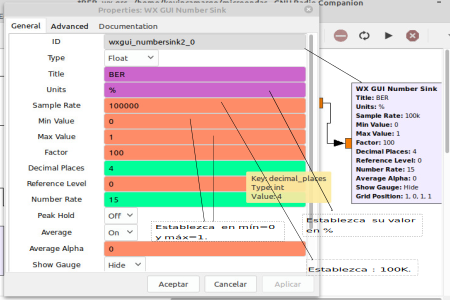
\includegraphics[width=1\textwidth]{Modulaciones_digitales/lab23/pdf/NimberSink.pdf}
\end{figure}
\begin{itemize}
    \item{Haga una conexion entre “Error Rate” y “Random Source” via Throtlle block.}
    \end{itemize}
\end{frame}

%_---------------------
%_---------------------

\begin{frame}
\begin{figure}[H]
\vspace{-3mm}
\centering
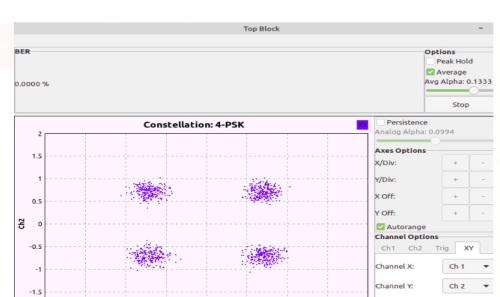
\includegraphics[width=1\textwidth]{Modulaciones_digitales/lab23/pdf/ErrorNulo.pdf}
\end{figure}
\end{frame}

%_---------------------
%_---------------------
%_---------------------
%_---------------------

\begin{frame}
\begin{figure}[H]
\vspace{-3mm}
\centering
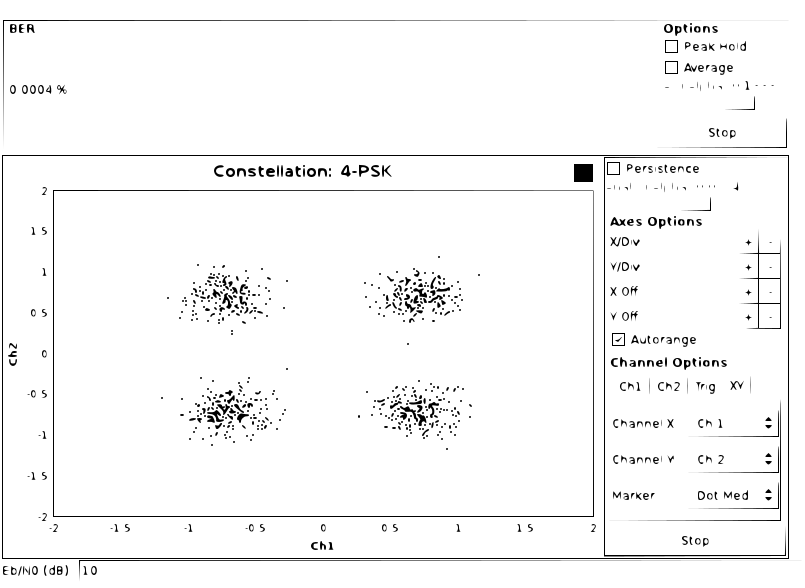
\includegraphics[width=1\textwidth]{Modulaciones_digitales/lab23/pdf/Captura.pdf}
\end{figure}
\end{frame}

%_---------------------
%_---------------------
